
\newcommand{\drawtruss}[1][1]{%
\begin{center}
\begin{tikzpicture}[scale=#1, every node/.style={scale=#1}]
\draw (0,0) node[left,magenta]{A} -- 
      (1,1.71) node[left,magenta]{D} -- 
      (2,0) node[above,magenta]{B} -- cycle;
\draw (2,0) -- node[left,magenta]{$5$} (3,1.71) -- node[above,magenta]{$4$} (1,1.71) -- cycle;
\draw (3,1.71) -- node[right,magenta]{$7$}  (4,0) -- node[above,magenta]{$6$} (2,0) -- cycle;
\draw[blue] (0,0) -- (0.25,-0.425) -- (-0.25,-0.425) -- cycle;
\draw[blue] (4,0) -- (4.25,-0.425) -- (3.75,-0.425) -- cycle;
\draw[thick,red,->] (2,0) --node[right]{10000 N} (2,-0.75);
\end{tikzpicture}
\end{center}
}


\begin{applicationActivities}

\begin{example}
In engineering, a \term{truss} is a structure designed from several beams
of material called \term{struts}, assembled to behave as a single object.

\begin{center}
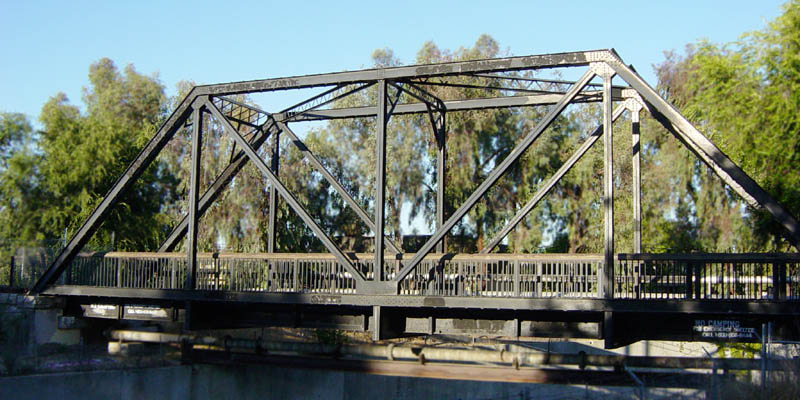
\includegraphics[width=0.8\linewidth]{media/truss.jpg}
\end{center}
\end{example}

\begin{activity}{10}
Consider the representation of a simple truss pictured below.
All of the seven struts are of equal length, affixed to two anchor points
with a \(10000 N\) load applied to the center of its base.

\drawtruss

Which of the following must hold?
\begin{enumerate}[a)]
\item All of the struts will experience compression.
\item All of the struts will experience tension.
\item Some of the struts will be compressed, and others will be tensioned.
\end{enumerate}
\end{activity}

\begin{observation}
Consider the truss pictured below with two fixed anchor points and a 10000 N load (assume all triangles are equilateral).
\drawtruss

The horizontal and vertical forces must balance at each  node.  For example, at the bottom left node there are 3 forces acting.
\begin{center}
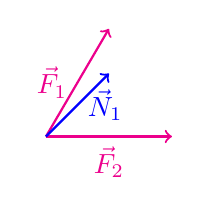
\begin{tikzpicture}[scale=0.8]
\draw [thick, magenta,->] (0,0) -- node[left]{$\vec{F}_1$} (1,1.71);
\draw [thick, magenta,->] (0,0) -- node[below]{$\vec{F}_2$} (2,0);
\draw [thick, blue,->] (0,0) -- node[right]{$\vec{N}_1$} (1,1);
\end{tikzpicture}
\end{center}

We adhere to the convention that a compression force on a strut is positive, while a negative force represents tension.
\end{observation}

\begin{observation}
\drawtruss[0.8]
We decompose the first node into vertical and horizontal forces:
\begin{multicols}{2}
\begin{center}
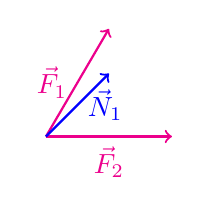
\begin{tikzpicture}[scale=0.8]
\draw [thick, magenta,->] (0,0) -- node[left]{$\vec{F}_1$} (1,1.71);
\draw [thick, magenta,->] (0,0) -- node[below]{$\vec{F}_2$} (2,0);
\draw [thick, blue,->] (0,0) -- node[right]{$\vec{N}_1$} (1,1);
\end{tikzpicture}
\end{center}
%
\begin{align*}
\vec{F}_1 &= F_1\begin{bmatrix} \cos(60^\circ) \\ \sin(60^\circ) \end{bmatrix} \\
\vec{N}_1 &= \begin{bmatrix} N_{1,h} \\ N_{1,v} \end{bmatrix}
\end{align*}
\end{multicols}

\begin{align*}
F_1 \sin(60^\circ)+N_{1,v} &= 0 \\
F_1 \cos(60^\circ)+N_{1,h}+F_2 &= 0
\end{align*}
\end{observation}

\begin{activity}{10}
Consider the truss pictured below with two fixed anchor points and a 10000 N load (assume all triangles are equilateral).
\drawtruss

From the bottom left node we obtained 2 equations in the four variables
\begin{itemize}
\item $F_{1}$ (compression force on strut one)
\item $N_{1,v}$ and $N_{1,h}$ (horizontal and vertical components of the normal force from the left anchor)
\item $F_2$ (compression force on strut 2).
\end{itemize}

\begin{subactivity}
Determine how many total equations there will be after accounting for all of the nodes, and and list all of the variables.  You do not need to actually determine all of the equations.
\end{subactivity}
\end{activity}


\begin{activity}{10}
\drawtruss[0.5]
The resulting system is
\scalebox{0.8}{
\begin{minipage}{0.8\linewidth}
\begin{alignat*}{12}
N_{1,v} &\,\,& &\,\,& &\,\,& &\,+\,& (\sin(60^\circ))F_1 &\,\,& &\,\,& &\,\,& &\,\,& &\,\,& &\,\,& &\,=\,& 0 \\
        &\,\,& N_{1,h} &\,\,& &\,\,& &\,+\,& (\cos(60^\circ))F_1 &\,+\,&F_2 &\,\,& &\,\,& &\,\,& &\,\,& &\,\,& &\,=\,& 0 \\
        &\,\,&         &\,\,& &\,\,& &\,-\,& (\sin(60^\circ))F_1 &\,\,& &\,-\,&(\sin(60^\circ)F_3 &\,\,& &\,\,& &\,\,& &\,\,& &\,=\,& 0 \\
        &\,\,&         &\,\,& &\,\,& &\,-\,& (\cos(60^\circ))F_1 &\,\,& &\,+\,&(\cos(60^\circ)F_3 &\,+\,&F_4 &\,\,& &\,\,& &\,\,& &\,=\,& 0 \\
        &\,\,&         &\,\,& &\,\,& &\,\,&                     &\,\,& &\,\,&(\sin(60^\circ)F_3 &\,\,& &\,+\,& (\sin(60^\circ))F_5&\,\,& &\,\,& &\,=\,& 10000 \\
        &\,\,&         &\,\,& &\,\,& &\,\,&                     &\,-\,& F_2&\,-\,&(\cos(60^\circ)F_3 &\,\,& &\,+\,& (\cos(60^\circ))F_5&\,+\,&F_6 &\,\,& &\,=\,& 0 \\
        &\,\,&         &\,\,& &\,\,& &\,\,&                     &\,\,& &\,\,&                   &\,\,& &\,-\,& (\sin(60^\circ))F_5&\,\,& &\,-\,& (\sin(60^\circ))F_7&\,=\,& 0 \\
        &\,\,&         &\,\,& &\,\,& &\,\,&                     &\,\,& &\,\,&                   &\,-\,&F_4 &\,-\,& (\cos(60^\circ))F_5&\,\,& &\,+\,& (\cos(60^\circ))F_7&\,=\,& 0 \\
        &\,\,&         &\,\,& N_{2,v} &\,\,& &\,\,&                     &\,\,& &\,\,&                   &\,\,& &\,\,&                    &\,\,& &\,+\,& (\sin(60^\circ))F_7&\,=\,& 0 \\
        &\,\,&         &\,\,& &\,\,&N_{2,h} &\,\,&                     &\,\,& &\,\,&                   &\,\,&    &\,\,&                    &\,-\,& F_6 &\,-\,& (\cos(60^\circ))F_7&\,=\,& 0
\end{alignat*}
\end{minipage}
}

Solve this system to determine which struts are compressed and which are in tension.
\end{activity}

\begin{observation}
\drawtruss[0.8]
The determined part of the solution is
\begin{align*}
N_{1,v}=N_{2,v}&=5000 \\
F_1=F_4=F_7&=-5882.4 \\
F_3=F_5&=5882.4
\end{align*}

So struts 1,4,7 are in tension, while struts 3 and 5 are compressed.

The forces on struts 2 and 6 (and the horizontal normal forces) are not strictly determined in this setting.
\end{observation}



\end{applicationActivities}
